\documentclass{beamer}
\usepackage{booktabs}
\usepackage{pdfpages}
\usepackage{mathtools}
\usepackage{enumerate}
\usepackage{multirow,tabularx}
\usepackage{booktabs}
\usepackage{pdfpages}
\usepackage{proof}
\usepackage{cancel}
\usepackage{chronology}
\usepackage{graphicx}
\usepackage{ulem}
\usepackage{amsmath}
\usepackage{amssymb}
\usepackage{color}

\PassOptionsToPackage{usenames,dvipsnames,svgnames}{xcolor}  
\usepackage{tikz}
\usepackage{tkz-graph}
\usetikzlibrary[positioning,arrows,automata]
\usepackage{wasysym}
\usepackage{proof}
\usepackage{cancel}
\usepackage{chronology}
\usepackage{graphicx}
\usepackage{ulem}
\usepackage{amsmath}
\usepackage{amssymb}
\usepackage{color}
\usepackage{xcolor}
\usepackage{soul}
%\usepackage{pstricks}
\setbeamertemplate{navigation symbols}{}

\newcommand{\myul}[2][blue]{\sethlcolor{#1}\hl{#2}\setulcolor{black}}

\newcommand<>{\cunderline}[3]{\only<#1>{#3}\only<#2>{\underline{#3}}}
\newcommand<>{\cem}[3]{\only<#1>{#3}\only<#2>{\ul{#3}}}
\newcommand<>{\cgray}[3]{\only<#1>{#3}\only<#2>{\textcolor{gray}{#3}}}
\newcommand<>{\colorize}[4]{\only<#1>{#4}\only<#2>{\textcolor{#3}{#4}}}

%\setbeamertemplate{navigation symbols}{}
\addtobeamertemplate{navigation symbols}{}{%
    \usebeamerfont{footline}%
    \usebeamercolor[fg]{footline}%
    \hspace{1em}%
    \insertframenumber/\inserttotalframenumber
}

\renewcommand{\em}{\itshape}

\mode<presentation>
% {
%   \usecolortheme{crane}
% %  \usetheme{Frankfurt}
% }
\mode<presentation>
{
  \usecolortheme{dove}
}

% \mode<presentation>
% {
% \useinnertheme[shadow=true]{rounded}
% \useoutertheme{infolines}
% \usecolortheme{dove}
% \setbeamerfont{block title}{size={}}
% }

\title[Ontologies]{Part 1: Ontologies and semantic similarity}

\author{Robert Hoehndorf}


\date{}

\begin{document}

\begin{frame}
  \titlepage
\end{frame}

\section{Introduction}

\begin{frame}
  \frametitle{Before the tutorial}
  See \url{https://github.com/bio-ontology-research-group/ontology-tutorial}:
  \begin{itemize}
  \item install Docker (e.g.: {\tt apt-get install docker})
  \item {\tt docker pull coolmaksat/embeddings:latest}
%  \item {\tt docker pull leechuck/ontology-ml:latest}
  \item {\tt docker run -i -t -p 8888:8888 coolmaksat/embeddings /bin/bash -c "jupyter notebook --notebook-dir=/home/borg/ontology-tutorial/ --ip='0.0.0.0' --port=8888 --no-browser --allow-root"}
  \end{itemize}
\end{frame}

\begin{frame}
  \frametitle{Learning goals}
  \begin{itemize}
  \item brief overview of ontologies in biomedicine
  \item semantic similarity with ontologies
  \item machine learning with ontologies as {\em features} (or
    background knowledge)
  \item unsupervised or supervised:
    \begin{itemize}
    \item here: mostly unsupervised {\em feature} learning
    \item ``deep'' learning
    \end{itemize}
  \item focus on existing tools and methods
    \begin{itemize}
    \item Jupyter Notebooks and code examples
    \end{itemize}
  \item not covered:
    \begin{itemize}
    \item learning ontologies (axioms, definitions) from data
    \item (most) natural language processing
    \item reasoning with ontologies
    \item learning on ``knowledge graphs''
    \item machine learning theory
    \end{itemize}
  \end{itemize}
\end{frame}

\begin{frame}
  \frametitle{Learning goals}
  Biomedical questions:
  \begin{itemize}
  \item diagnosing rare disease
  \item finding functionally similar proteins
  \item relying on heterogeneous data integration
    \begin{itemize}
    \item from different databases
    \item model organisms
    \end{itemize}
  \end{itemize}
\end{frame}

\begin{frame}
  \frametitle{Agenda}
  \begin{itemize}
  \item Introduction: ontologies and graphs
  \item Semantic similarity
  \item Machine learning:
    \begin{itemize}
    \item syntactic
    \item graph-based
    \item model-theoretic
    \end{itemize}
  \end{itemize}
\end{frame}


\section{Ontologies and the Semantic Web}

\begin{frame}
  \frametitle{Ontologies, machine learning, and AI}
  \begin{itemize}
  \item ontologies are ubiquitous in biomedical research
  \item rich formal characterization (axioms)
  \item how can they be used for (predictive) data analysis?
    \begin{itemize}
    \item ``fuzzy'', similarity-based search
    \item background knowledge in machine learning
    \end{itemize}
  \end{itemize}
\end{frame}

\begin{frame}
  \frametitle{Ontologies}
  \centerline{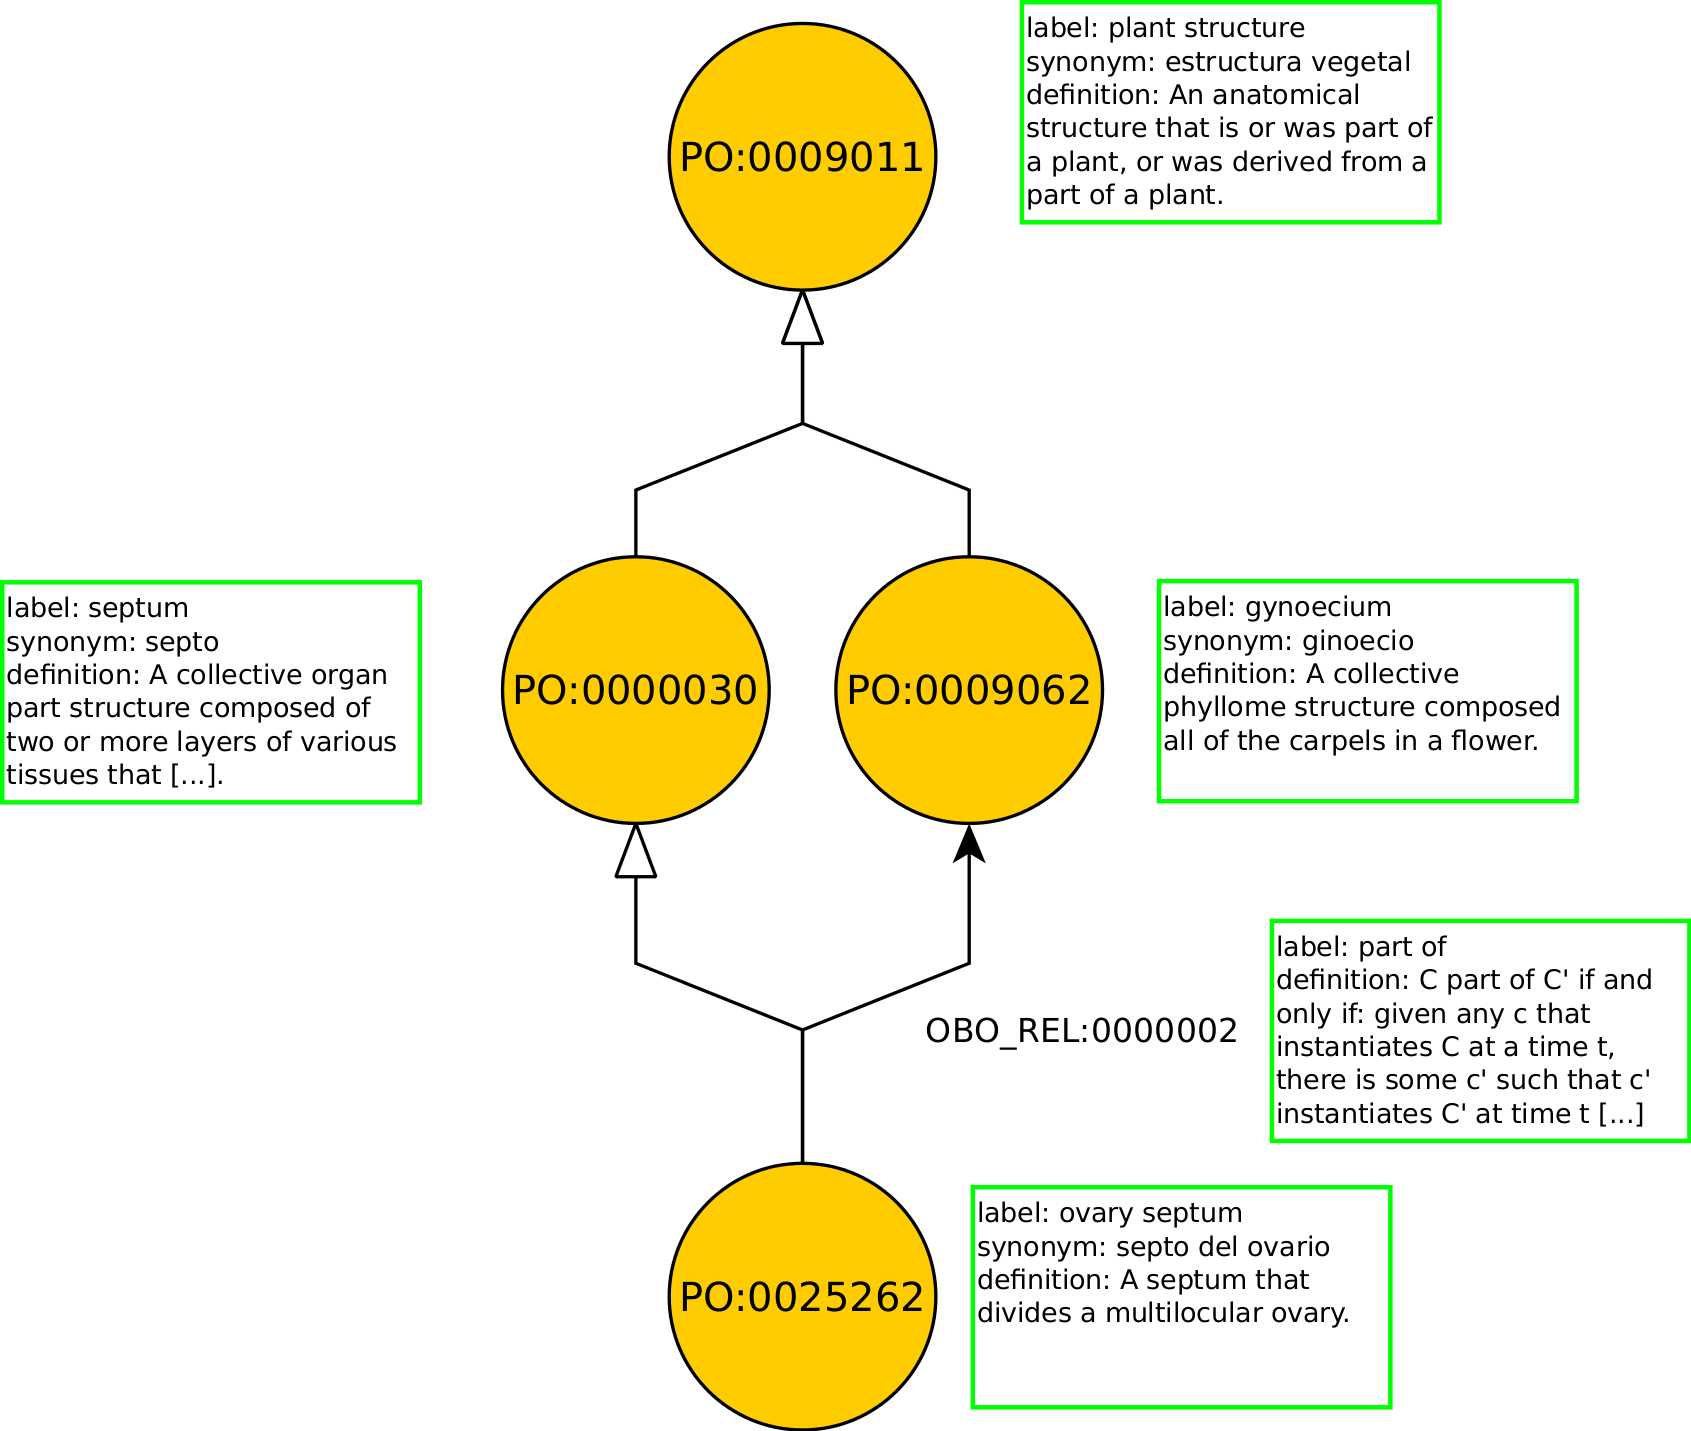
\includegraphics[height=.8\textheight]{plant-ontology-sample.png}}

\end{frame}

\begin{frame}
  \frametitle{Ontologies for data integration}

  \begin{itemize}
  \item standard identifiers (IRIs)
  \item labels of classes and relations
  \item human-readable descriptions
  \item axioms
  \end{itemize}
  
\end{frame}

\begin{frame}
  \frametitle{Ontologies provide domain knowledge}

  \centerline{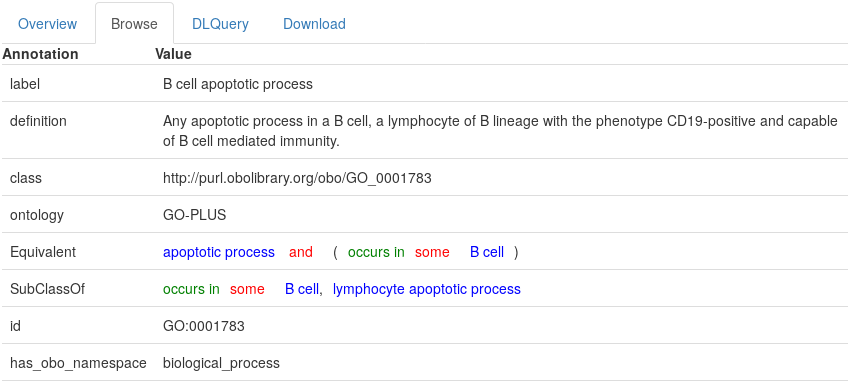
\includegraphics[width=.85\textwidth]{bcellapoptosis.png}}
  
  
\end{frame}

\begin{frame}
  \frametitle{The Semantic Web}
  \centerline{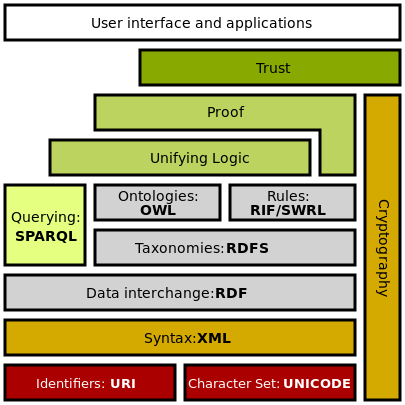
\includegraphics[width=.6\textwidth]{semwebstack.png}}
\end{frame}

\begin{frame}
  \frametitle{Manchester OWL Syntax}
  \begin{table}[ht]
    \centering
    \begin{tabular}{|l|l|l|}
      DL Syntax & Manchester Syntax & Example \\
      \hline
      $C \sqcap D$ & C and D & Human and Male \\
      $C \sqcup D$ & C or D & Male or Female \\
      $\neg C$ & not C & not Male \\
      $\exists R.C$ & R some C & hasChild some Human \\
      $\forall R.C$ & R only C & hasChild only Human \\
      $(\geq n R.C)$ & R min n C & hasChild min 1 Human \\
      $(\leq n R.C)$ & R max n C & hasChild max 1 Human \\
      $(= n R.C)$ & R exactly n C & hasChild exactly 1 Human \\
      $\{a\} \sqcup \{b\} \sqcup ...$ & \{a b ...\} & \{John Robert
                                                      Mary\} \\
      \hline
    \end{tabular}
  \end{table}
\end{frame}

\begin{frame}
  \frametitle{Reasoning with ontologies}
  \begin{itemize}
  \item {\tt 'B cell apoptosis' EquivalentTo: apoptosis and 'occurs
      in' some 'B cell'}
  \item {\tt 'lymphocyte apoptosis' EquivalentTo: apoptosis and 'occurs
      in' some lymphocyte}
  \item {\tt 'B cell' SubClassOf: lymphocyte}
    \pause
  \item {\tt 'B cell apoptosis' SubClassOf: 'lymphocyte apoptosis'}
  \end{itemize}
  
\end{frame}

\begin{frame}
  \frametitle{Reasoning with phenotype ontologies}
  Phenotype ontology:
  \begin{itemize}
  \item A phenotype is a quality that inheres in its bearer:
    \begin{itemize}
    \item Enlarged heart:
      $Enlarged(x) \land \exists y ( inheresIn(x,y) \land Heart(y))$
    \item in DL: $Enlarged \sqcap \exists inheresIn.Heart$
  \item Enlarged: reuse an ontology of qualities (PATO)
  \item Heart: reuse ontology of (human, mammalian) anatomy
  \end{itemize}
\end{itemize}
\end{frame}

\begin{frame}
  \frametitle{UberPheno, PhenomeNET}
  \centerline{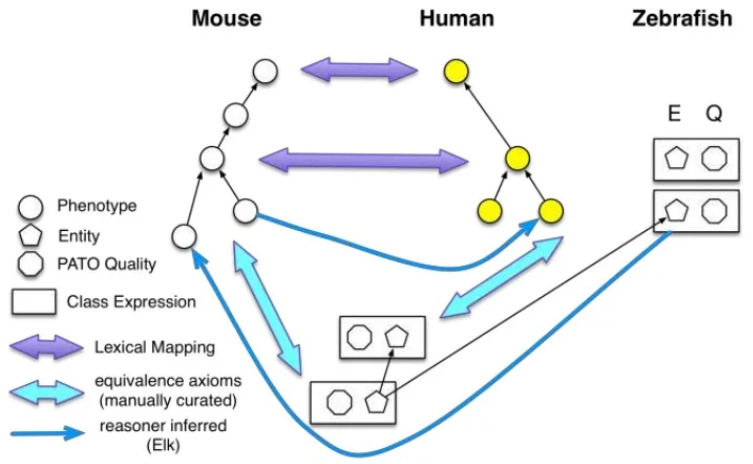
\includegraphics[width=.8\textwidth]{uberpheno.png}}
\end{frame}

\begin{frame}
  \frametitle{BLAST-like search over phenotypes}
  Using ontologies and reasoning, we can
  \begin{enumerate}
  \item describe phenotypes computationally
    \begin{itemize}
    \item morphology
    \item function
    \item $\Rightarrow$ ontologies
    \end{itemize}
  \item integrate/compare phenotypes {\em within and between species}
    (to overcome limitations in phenotype data)
    \begin{itemize}
    \item homologous organ structures
    \item related/identical function
    \item $\Rightarrow$ ontologies and automated reasoning
    \end{itemize}
  \item measure phenotypic similarity
    \begin{itemize}
    \item use morphological or functional similarity
    \item similarity in attribute values
    \item $\Rightarrow$ semantic similarity, machine learning
    \end{itemize}
  \end{enumerate}
\end{frame}

\section{Ontologies and graphs}

\begin{frame}
  \frametitle{Other questions we want to answer}
  \begin{itemize}
  \item Are cyclin dependent kinases {\em functionally} more similar
    to lipid kinases or to riboflavin kinases? How about {\em
      phenotypically}?
    \pause
  \item Which protein in the {\em mouse} is functionally most similar
    to the zebrafish {\em gustducin} protein?
    \pause
  \item Which mouse knockout resembles {\em Bardet-Biedl Syndrome 8}?
    \pause
  \item Are there mouse knockouts that resemble the side effects of
    diclofenac?
    \pause
  \item Which genetic disease produces similar symptoms to ebola?
    \pause
  \item Does functional similarity correlate with phenotypic similarity?
  \end{itemize}
\end{frame}

\begin{frame}
  \frametitle{Ontologies and graphs}
  \begin{itemize}
  \item semantic similarity measures can be graph-based,
    feature-based, or model-based
  \item we may need to generate graphs from ontologies
    \begin{itemize}
    \item remember: ontologies are sets of axioms
    \item {\em subclass} axioms are easy
    \item how about more complex axioms?
    \end{itemize}
  \item solution: define relational patterns
  \end{itemize}
\end{frame}

\begin{frame}
  \frametitle{Relations as patterns}
  \begin{itemize}
  \item {\tt X SubClassOf: Y}: $X \xrightarrow{\text{is-a}} Y$
  \item {\tt X SubClassOf: part-of some Y}: $X \xrightarrow{\text{part-of}} Y$
  \item {\tt X SubClassOf: regulates some Y}: $X \xrightarrow{\text{regulates}} Y$
  \item {\tt X DisjointWith: Y}: $X \xleftrightarrow{\text{disjoint}} Y$
  \item {\tt X EquivalentTo: Y}: $X \xleftrightarrow{\equiv} Y$, $\{X,Y\}$
  \end{itemize}
\end{frame}

\begin{frame}
  \frametitle{Relations as patterns}
  \centerline{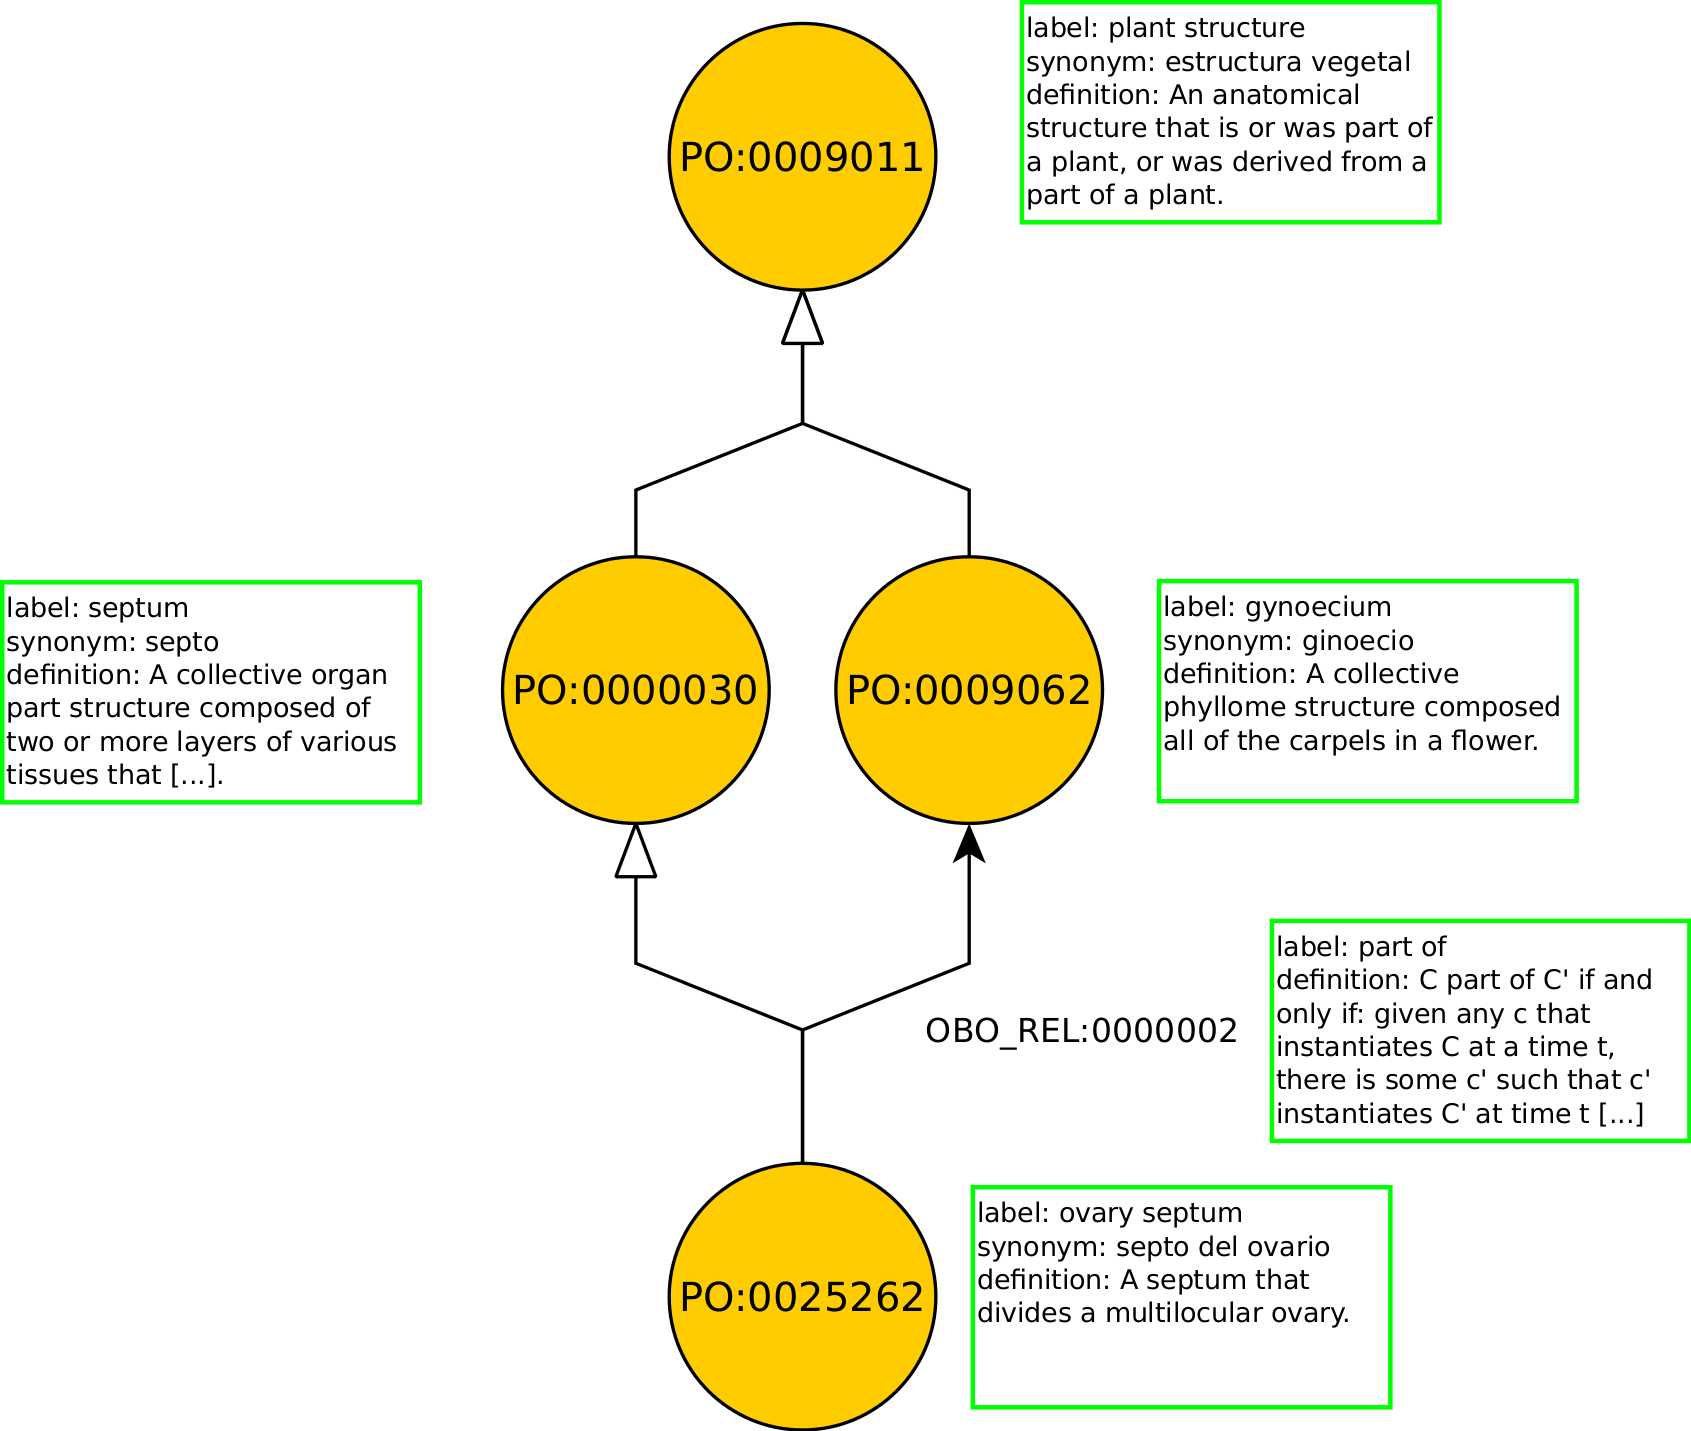
\includegraphics[height=.8\textheight]{plant-ontology-sample.png}}
\end{frame}

\section{Semantic Similarity}

\begin{frame}
  Semantic similarity
  \begin{itemize}
  \item We want to use {\em  background knowledge} in ontologies to
    \begin{itemize}
    \item determine similarity between classes,
    \item instances,
    \item and entities with ontology annotations
    \end{itemize}
  \end{itemize}
\end{frame}


\begin{frame}
  \frametitle{How to measure similarity?}
  \begin{itemize}
  \item semantic similarity measures similarity between classes
  \item semantic similarity measures similarity between instances of classes
  \item semantic similarity measures similarity between entities
    {\em annotated} with classes
  \item $\Rightarrow$ reduce all of this to similarity between classes
  \end{itemize}
\end{frame}

\begin{frame}
  \frametitle{How to measure similarity?}
  What properties do we want in a similarity measure?
  \\
  A function $sim: D \times D$ is a similarity on $D$ if, for
  all $x, y \in D$, the function $sim$ is:  \begin{itemize}
    \pause
  \item non-negative: $sim(x,y) \geq 0$ for all $x, y$
    \pause
  \item symmetric: $sim(x,y) = sim(y,x)$
    \pause
  \item reflexive: $sim(x,x) = max_D$
    \pause
    \begin{itemize}
    \item weaker form: $sim(x,x) > sim(x,y)$ for all $x \not= y$
    \end{itemize}
    \pause
  \item $sim(x,x) > sim(x,y)$ for $x\not= y$
    \pause
  \item $sim$ is a {\em normalized} similarity measure if it has
    values in $[0,1]$
  \end{itemize}
\end{frame}

\begin{frame}
  \frametitle{How to measure similarity?}
  \begin{columns}
    \begin{column}{.6\textwidth}
      {\tiny
        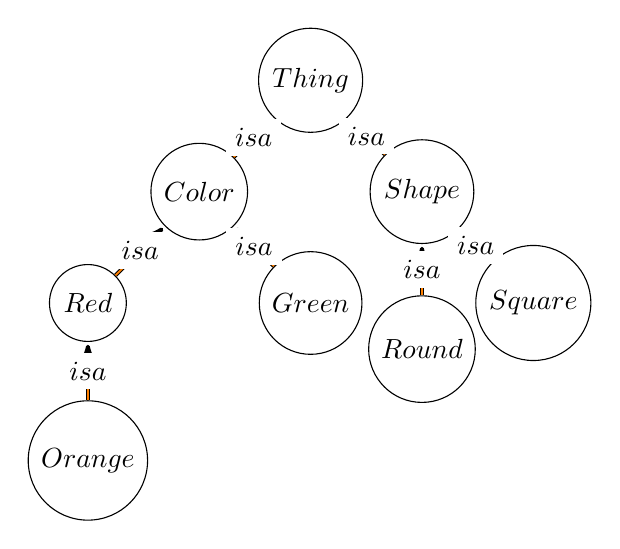
\begin{tikzpicture}[>=stealth',shorten >=1pt,node distance=2cm,on grid,initial/.style    ={}]
          \node[state]          (A)                        {$Thing$};
          \node[state]          (B) [below left =of A]    {$Color$};
          \node[state]          (C) [below right =of A]    {$Shape$};
          \node[state]          (D) [below left =of B]    {$Red$};
          \node[state]          (H) [below right =of B]    {$Green$};
          \node[state]          (E) [below  =of D]    {$Orange$};
          \node[state]          (F) [below =of C]    {$Round$};
          \node[state]          (G) [below right =of C]    {$Square$};
          \tikzset{mystyle/.style={->,double=orange}} 
          \tikzset{every node/.style={fill=white}} 
          \path (B)     edge [mystyle]    node   {$isa$} (A)
          (C)     edge [mystyle]    node   {$isa$} (A) 
          (D)     edge [mystyle]    node   {$isa$} (B)
          (H)     edge [mystyle]    node   {$isa$} (B)
          (E)     edge [mystyle]    node   {$isa$} (D)
          (F)     edge [mystyle]    node   {$isa$} (C)
          (G)     edge [mystyle]    node   {$isa$} (C);
          \tikzset{mystyle/.style={<->,double=orange}}   
          \tikzset{mystyle/.style={<->,relative=true,in=0,out=60,double=orange}}
        \end{tikzpicture}
      }
    \end{column}
    \begin{column}{.4\textwidth}
      \begin{itemize}
        \pause
      \item distance on shortest path (Rada {\em et al.}, 1989)
        \pause
      \item $dist_{Rada}(u,v) = sp(u, isa, v)$
        \pause
      \item $sim_{Rada}(u,v) = \frac{1}{dist_{Rada}(u,v) + 1}$
      \end{itemize}
    \end{column}
  \end{columns}
\end{frame}

\begin{frame}
  \frametitle{How to measure similarity?}
  \begin{columns}
    \begin{column}{.6\textwidth}
      {\tiny
        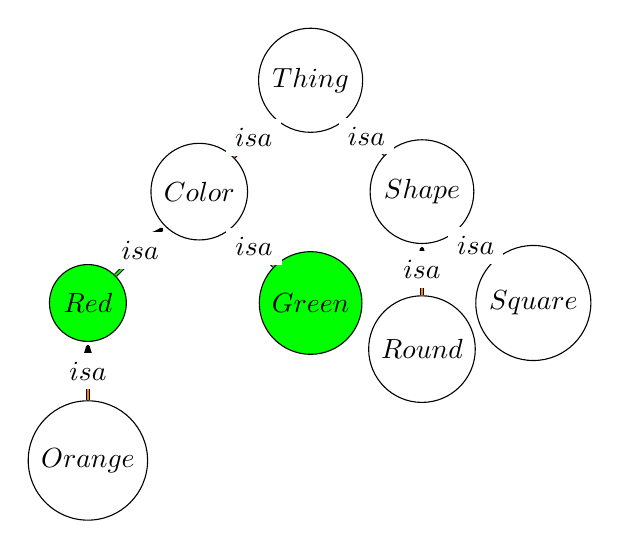
\begin{tikzpicture}[>=stealth',shorten >=1pt,node distance=2cm,on grid,initial/.style    ={}]
          \node[state]          (A)                        {$Thing$};
          \node[state]          (B) [below left =of A]    {$Color$};
          \node[state]          (C) [below right =of A]    {$Shape$};
          \node[state, fill=green]          (D) [below left =of B]    {$Red$};
          \node[state, fill=green]          (H) [below right =of B]    {$Green$};
          \node[state]          (E) [below  =of D]    {$Orange$};
          \node[state]          (F) [below =of C]    {$Round$};
          \node[state]          (G) [below right =of C]    {$Square$};
          \tikzset{mystyle/.style={->,double=orange}} 
          \tikzset{highlight/.style={->,double=green}} 
          \tikzset{every node/.style={fill=white}}
          \path (B)     edge [mystyle]    node   {$isa$} (A)
          (C)     edge [mystyle]    node   {$isa$} (A) 
          (D)     edge [highlight]    node   {$isa$} (B)
          (H)     edge [highlight]    node   {$isa$} (B)
          (E)     edge [mystyle]    node   {$isa$} (D)
          (F)     edge [mystyle]    node   {$isa$} (C)
          (G)     edge [mystyle]    node   {$isa$} (C);
          \tikzset{mystyle/.style={<->,double=orange}}   
          \tikzset{mystyle/.style={<->,relative=true,in=0,out=60,double=orange}}
        \end{tikzpicture}
      }
    \end{column}
    \begin{column}{.4\textwidth}
      \begin{itemize}
      \item distance on shortest path
        \pause
       \item distance(green, red) = 2
       \item $sim_{Rada}(green, red) = \frac{1}{3}$
      \end{itemize}
    \end{column}
  \end{columns}
\end{frame}

\begin{frame}
  \frametitle{How to measure similarity?}
  \begin{columns}
    \begin{column}{.6\textwidth}
      {\tiny
        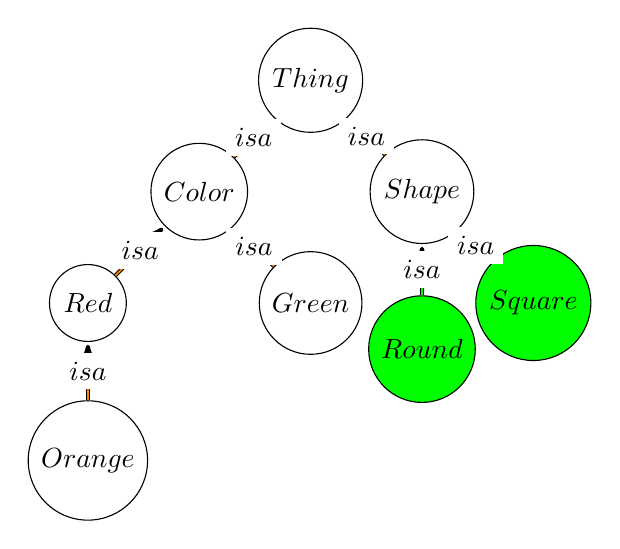
\begin{tikzpicture}[>=stealth',shorten >=1pt,node distance=2cm,on grid,initial/.style    ={}]
          \node[state]          (A)                        {$Thing$};
          \node[state]          (B) [below left =of A]    {$Color$};
          \node[state]          (C) [below right =of A]    {$Shape$};
          \node[state]          (D) [below left =of B]    {$Red$};
          \node[state]          (H) [below right =of B]    {$Green$};
          \node[state]          (E) [below  =of D]    {$Orange$};
          \node[state, fill=green]          (F) [below =of C]    {$Round$};
          \node[state, fill=green]          (G) [below right =of C]    {$Square$};
          \tikzset{mystyle/.style={->,double=orange}} 
          \tikzset{highlight/.style={->,double=green}} 
          \tikzset{every node/.style={fill=white}}
          \path (B)     edge [mystyle]    node   {$isa$} (A)
          (C)     edge [mystyle]    node   {$isa$} (A) 
          (D)     edge [mystyle]    node   {$isa$} (B)
          (H)     edge [mystyle]    node   {$isa$} (B)
          (E)     edge [mystyle]    node   {$isa$} (D)
          (F)     edge [highlight]    node   {$isa$} (C)
          (G)     edge [highlight]    node   {$isa$} (C);
          \tikzset{mystyle/.style={<->,double=orange}}   
          \tikzset{mystyle/.style={<->,relative=true,in=0,out=60,double=orange}}
        \end{tikzpicture}
      }
    \end{column}
    \begin{column}{.4\textwidth}
      \begin{itemize}
       \item distance on shortest path
       \item distance(square, round) = 2
       \item $sim_{Rada}(square, round) = \frac{1}{3}$
      \end{itemize}
    \end{column}
  \end{columns}
\end{frame}

\begin{frame}
  \frametitle{How to measure similarity?}
  \begin{columns}
    \begin{column}{.6\textwidth}
      {\tiny
        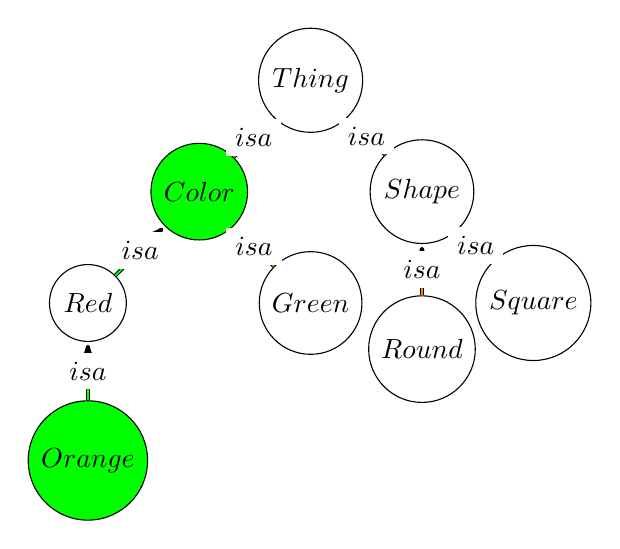
\begin{tikzpicture}[>=stealth',shorten >=1pt,node distance=2cm,on grid,initial/.style    ={}]
          \node[state]          (A)                        {$Thing$};
          \node[state, fill=green]          (B) [below left =of A]    {$Color$};
          \node[state]          (C) [below right =of A]    {$Shape$};
          \node[state]          (D) [below left =of B]    {$Red$};
          \node[state]          (H) [below right =of B]    {$Green$};
          \node[state, fill=green]          (E) [below  =of D]    {$Orange$};
          \node[state]          (F) [below =of C]    {$Round$};
          \node[state]          (G) [below right =of C]    {$Square$};
          \tikzset{mystyle/.style={->,double=orange}} 
          \tikzset{highlight/.style={->,double=green}} 
          \tikzset{every node/.style={fill=white}}
          \path (B)     edge [mystyle]    node   {$isa$} (A)
          (C)     edge [mystyle]    node   {$isa$} (A) 
          (D)     edge [highlight]    node   {$isa$} (B)
          (H)     edge [mystyle]    node   {$isa$} (B)
          (E)     edge [highlight]    node   {$isa$} (D)
          (F)     edge [mystyle]    node   {$isa$} (C)
          (G)     edge [mystyle]    node   {$isa$} (C);
          \tikzset{mystyle/.style={<->,double=orange}}   
          \tikzset{mystyle/.style={<->,relative=true,in=0,out=60,double=orange}}
        \end{tikzpicture}
      }
    \end{column}
    \begin{column}{.4\textwidth}
      \begin{itemize}
       \item distance on shortest path
       \item distance(orange, color) = 2
       \item $sim_{Rada}(orange, color) = \frac{1}{3}$
      \end{itemize}
    \end{column}
  \end{columns}
\end{frame}

\begin{frame}
  \frametitle{How to measure similarity?}
  \begin{itemize}
  \item shortest path is not always intuitive
    \pause
  \item we need a way to determine {\em specificity} of a class
    \begin{itemize}
    \item number of ancestors
    \item number of children
    \item information content
    \end{itemize}
    \pause
  \item {\em density} of a branch in the ontology
    \begin{itemize}
    \item number of siblings
    \item information content
    \end{itemize}
    \pause
  \item account for different edge types
    \begin{itemize}
    \item non-uniform edge weighting
    \end{itemize}
  \end{itemize}
\end{frame}

\begin{frame}
  \frametitle{How to measure similarity}
  \begin{itemize}
  \item term specificity measure $\sigma: C \mapsto \mathbb{R}$:
    \begin{itemize}
    \item $x \sqsubseteq y \rightarrow \sigma(x) \geq \sigma(y)$
    \end{itemize}
    \pause
  \item intrinsic:
    \begin{itemize}
    \item $\sigma(x) = f(depth(x))$
    \item $\sigma(x) = f(A(x))$ (for ancestors $A(x)$)
    \item $\sigma(x) = f(D(x))$ (for descendants $D(x)$)
    \item many more, e.g., Zhou et al.: $\sigma(x) = k \cdot \Big( 1-\frac{\log
        |D(x)|}{\log |C|} \Big) + (1-k) \frac{\log depth(x)}{\log
        depth(G_T)} $
    \end{itemize}
    \pause
  \item extrinsic:
    \begin{itemize}
    \item $\sigma(x)$ defined as a function of instances (or annotations) $I$
      \begin{itemize}
      \item note: the number of instances monotonically decreases with
        increasing depth in taxonomies
      \end{itemize}
    \item Resnik 1995: $eIC_{Resnik}(x) = -\log p(x)$ (with $p(x) =
      \frac{|I(x)|}{|I|}$)
      \begin{itemize}
      \item in biology, one of the most popular specificity measure when
        annotations are present
      \end{itemize}
    \end{itemize}
  \end{itemize}
\end{frame}

\begin{frame}
  \frametitle{How to measure similarity?}
  \begin{columns}
    \begin{column}{.6\textwidth}
      {\tiny
        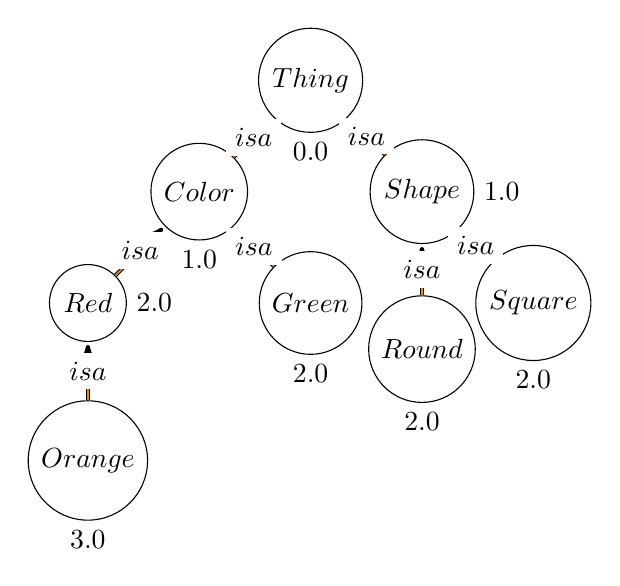
\begin{tikzpicture}[>=stealth',shorten >=1pt,node distance=2cm,on grid,initial/.style    ={}]
          \node[state,label=below:$0.0$]          (A)                        {$Thing$};
          \node[state,label=below:$1.0$]          (B) [below left =of A]    {$Color$};
          \node[state,label=right:$1.0$]          (C) [below right =of A]    {$Shape$};
          \node[state,label=right:$2.0$]          (D) [below left =of B]    {$Red$};
          \node[state,label=below:$2.0$]          (H) [below right =of B]    {$Green$};
          \node[state,label=below:$3.0$]          (E) [below  =of D]    {$Orange$};
          \node[state,label=below:$2.0$]          (F) [below =of C]    {$Round$};
          \node[state,label=below:$2.0$]          (G) [below right =of C]    {$Square$};
          \tikzset{mystyle/.style={->,double=orange}} 
          \tikzset{highlight/.style={->,double=green}} 
          \tikzset{every node/.style={fill=white}}
          \path (B)     edge [mystyle]    node   {$isa$} (A)
          (C)     edge [mystyle]    node   {$isa$} (A) 
          (D)     edge [mystyle]    node   {$isa$} (B)
          (H)     edge [mystyle]    node   {$isa$} (B)
          (E)     edge [mystyle]    node   {$isa$} (D)
          (F)     edge [mystyle]    node   {$isa$} (C)
          (G)     edge [mystyle]    node   {$isa$} (C);
          \tikzset{mystyle/.style={<->,double=orange}}   
          \tikzset{mystyle/.style={<->,relative=true,in=0,out=60,double=orange}}
        \end{tikzpicture}
      }
    \end{column}
    \begin{column}{.4\textwidth}
      \begin{itemize}
      \item Resnik 1995: similarity between $x$ and $y$ is the
        information content of the {\em most informative common
          ancestor}
      \end{itemize}
    \end{column}
  \end{columns}
\end{frame}

\begin{frame}
  \frametitle{How to measure similarity?}
  \begin{columns}
    \begin{column}{.6\textwidth}
      {\tiny
        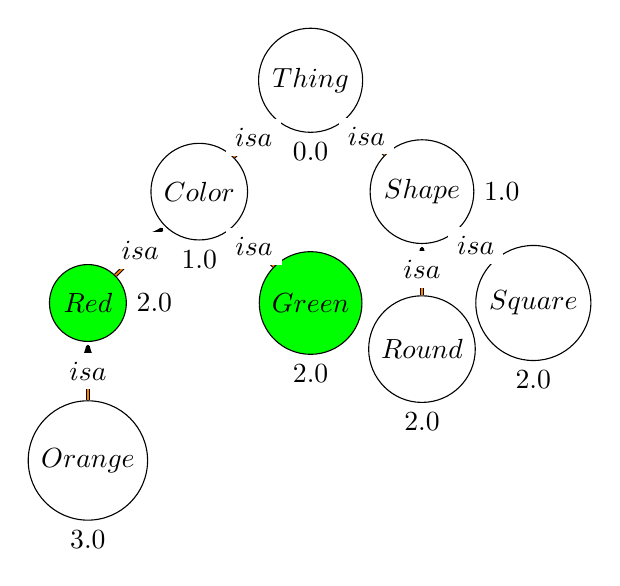
\begin{tikzpicture}[>=stealth',shorten >=1pt,node distance=2cm,on grid,initial/.style    ={}]
          \node[state,label=below:$0.0$]          (A)                        {$Thing$};
          \node[state,label=below:$1.0$]          (B) [below left =of A]    {$Color$};
          \node[state,label=right:$1.0$]          (C) [below right =of A]    {$Shape$};
          \node[state,fill=green,label=right:$2.0$]          (D) [below left =of B]    {$Red$};
          \node[state,fill=green,label=below:$2.0$]          (H) [below right =of B]    {$Green$};
          \node[state,label=below:$3.0$]          (E) [below  =of D]    {$Orange$};
          \node[state,label=below:$2.0$]          (F) [below =of C]    {$Round$};
          \node[state,label=below:$2.0$]          (G) [below right =of C]    {$Square$};
          \tikzset{mystyle/.style={->,double=orange}} 
          \tikzset{highlight/.style={->,double=green}} 
          \tikzset{every node/.style={fill=white}}
          \path (B)     edge [mystyle]    node   {$isa$} (A)
          (C)     edge [mystyle]    node   {$isa$} (A) 
          (D)     edge [mystyle]    node   {$isa$} (B)
          (H)     edge [mystyle]    node   {$isa$} (B)
          (E)     edge [mystyle]    node   {$isa$} (D)
          (F)     edge [mystyle]    node   {$isa$} (C)
          (G)     edge [mystyle]    node   {$isa$} (C);
          \tikzset{mystyle/.style={<->,double=orange}}   
          \tikzset{mystyle/.style={<->,relative=true,in=0,out=60,double=orange}}
        \end{tikzpicture}
      }
    \end{column}
    \begin{column}{.4\textwidth}
      \begin{itemize}
      \item Resnik 1995: similarity between $x$ and $y$ is the
        information content of the {\em most informative common
          ancestor}
      \end{itemize}
    \end{column}
  \end{columns}
\end{frame}

\begin{frame}
  \frametitle{How to measure similarity?}
  \begin{columns}
    \begin{column}{.6\textwidth}
      {\tiny
        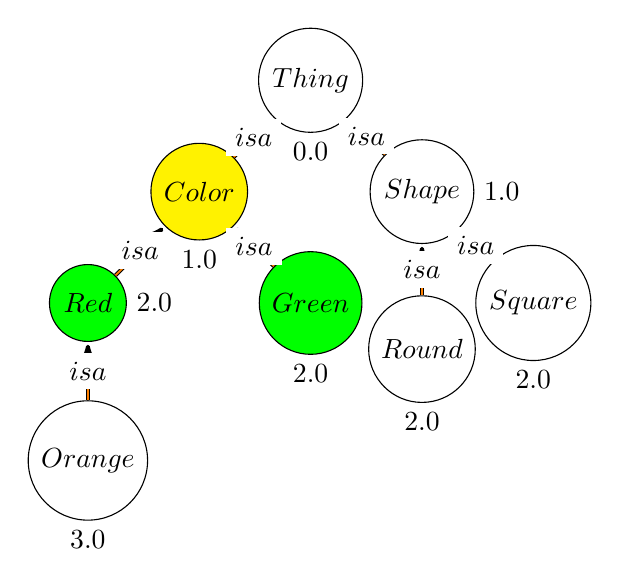
\begin{tikzpicture}[>=stealth',shorten >=1pt,node distance=2cm,on grid,initial/.style    ={}]
          \node[state,label=below:$0.0$]          (A)                        {$Thing$};
          \node[state,fill=yellow,label=below:$1.0$]          (B) [below left =of A]    {$Color$};
          \node[state,label=right:$1.0$]          (C) [below right =of A]    {$Shape$};
          \node[state,fill=green,label=right:$2.0$]          (D) [below left =of B]    {$Red$};
          \node[state,fill=green,label=below:$2.0$]          (H) [below right =of B]    {$Green$};
          \node[state,label=below:$3.0$]          (E) [below  =of D]    {$Orange$};
          \node[state,label=below:$2.0$]          (F) [below =of C]    {$Round$};
          \node[state,label=below:$2.0$]          (G) [below right =of C]    {$Square$};
          \tikzset{mystyle/.style={->,double=orange}} 
          \tikzset{highlight/.style={->,double=green}} 
          \tikzset{every node/.style={fill=white}}
          \path (B)     edge [mystyle]    node   {$isa$} (A)
          (C)     edge [mystyle]    node   {$isa$} (A) 
          (D)     edge [mystyle]    node   {$isa$} (B)
          (H)     edge [mystyle]    node   {$isa$} (B)
          (E)     edge [mystyle]    node   {$isa$} (D)
          (F)     edge [mystyle]    node   {$isa$} (C)
          (G)     edge [mystyle]    node   {$isa$} (C);
          \tikzset{mystyle/.style={<->,double=orange}}   
          \tikzset{mystyle/.style={<->,relative=true,in=0,out=60,double=orange}}
        \end{tikzpicture}
      }
    \end{column}
    \begin{column}{.4\textwidth}
      \begin{itemize}
      \item Resnik 1995: similarity between $x$ and $y$ is the
        information content of the {\em most informative common
          ancestor}
      \end{itemize}
    \end{column}
  \end{columns}
\end{frame}

\begin{frame}
  \frametitle{How to measure similarity?}
  \begin{columns}
    \begin{column}{.6\textwidth}
      {\tiny
        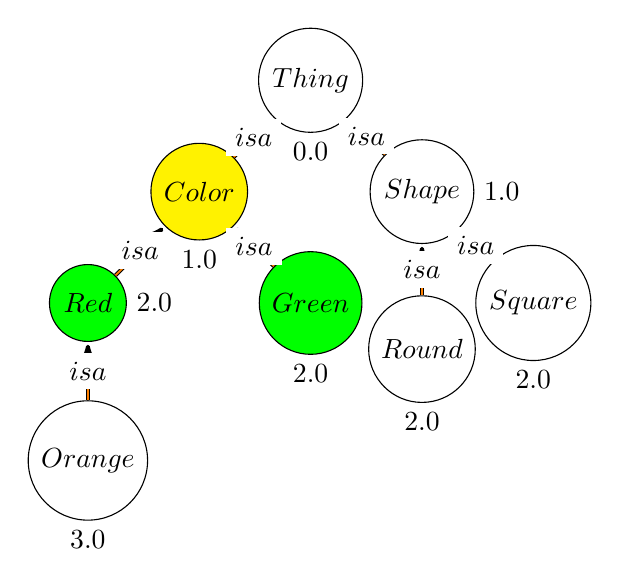
\begin{tikzpicture}[>=stealth',shorten >=1pt,node distance=2cm,on grid,initial/.style    ={}]
          \node[state,label=below:$0.0$]          (A)                        {$Thing$};
          \node[state,fill=yellow,label=below:$1.0$]          (B) [below left =of A]    {$Color$};
          \node[state,label=right:$1.0$]          (C) [below right =of A]    {$Shape$};
          \node[state,fill=green,label=right:$2.0$]          (D) [below left =of B]    {$Red$};
          \node[state,fill=green,label=below:$2.0$]          (H) [below right =of B]    {$Green$};
          \node[state,label=below:$3.0$]          (E) [below  =of D]    {$Orange$};
          \node[state,label=below:$2.0$]          (F) [below =of C]    {$Round$};
          \node[state,label=below:$2.0$]          (G) [below right =of C]    {$Square$};
          \tikzset{mystyle/.style={->,double=orange}} 
          \tikzset{highlight/.style={->,double=green}} 
          \tikzset{every node/.style={fill=white}}
          \path (B)     edge [mystyle]    node   {$isa$} (A)
          (C)     edge [mystyle]    node   {$isa$} (A) 
          (D)     edge [mystyle]    node   {$isa$} (B)
          (H)     edge [mystyle]    node   {$isa$} (B)
          (E)     edge [mystyle]    node   {$isa$} (D)
          (F)     edge [mystyle]    node   {$isa$} (C)
          (G)     edge [mystyle]    node   {$isa$} (C);
          \tikzset{mystyle/.style={<->,double=orange}}   
          \tikzset{mystyle/.style={<->,relative=true,in=0,out=60,double=orange}}
        \end{tikzpicture}
      }
    \end{column}
    \begin{column}{.4\textwidth}
      \begin{itemize}
      \item Resnik 1995: similarity between $x$ and $y$ is the
        information content of the {\em most informative common
          ancestor}
        \item $sim_{Resnik}(Green, Red) = 1.0$
      \end{itemize}
    \end{column}
  \end{columns}
\end{frame}

\begin{frame}
  \frametitle{How to measure similarity?}
  \begin{columns}
    \begin{column}{.6\textwidth}
      {\tiny
        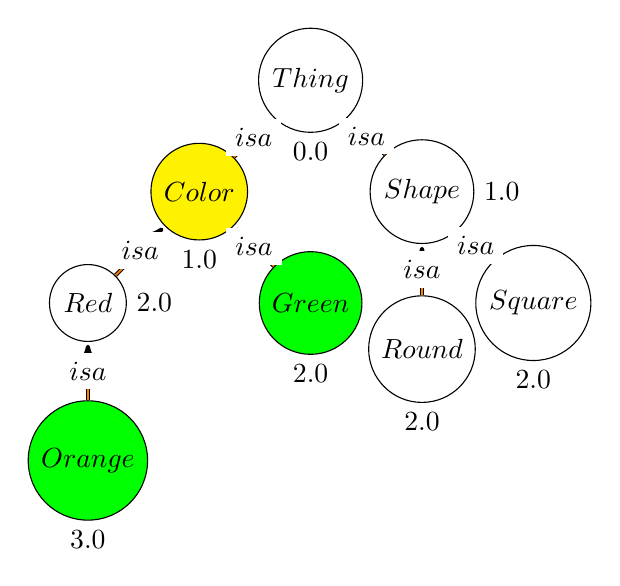
\begin{tikzpicture}[>=stealth',shorten >=1pt,node distance=2cm,on grid,initial/.style    ={}]
          \node[state,label=below:$0.0$]          (A)                        {$Thing$};
          \node[state,fill=yellow,label=below:$1.0$]          (B) [below left =of A]    {$Color$};
          \node[state,label=right:$1.0$]          (C) [below right =of A]    {$Shape$};
          \node[state,label=right:$2.0$]          (D) [below left =of B]    {$Red$};
          \node[state,fill=green,label=below:$2.0$]          (H) [below right =of B]    {$Green$};
          \node[state,fill=green,label=below:$3.0$]          (E) [below  =of D]    {$Orange$};
          \node[state,label=below:$2.0$]          (F) [below =of C]    {$Round$};
          \node[state,label=below:$2.0$]          (G) [below right =of C]    {$Square$};
          \tikzset{mystyle/.style={->,double=orange}} 
          \tikzset{highlight/.style={->,double=green}} 
          \tikzset{every node/.style={fill=white}}
          \path (B)     edge [mystyle]    node   {$isa$} (A)
          (C)     edge [mystyle]    node   {$isa$} (A) 
          (D)     edge [mystyle]    node   {$isa$} (B)
          (H)     edge [mystyle]    node   {$isa$} (B)
          (E)     edge [mystyle]    node   {$isa$} (D)
          (F)     edge [mystyle]    node   {$isa$} (C)
          (G)     edge [mystyle]    node   {$isa$} (C);
          \tikzset{mystyle/.style={<->,double=orange}}   
          \tikzset{mystyle/.style={<->,relative=true,in=0,out=60,double=orange}}
        \end{tikzpicture}
      }
    \end{column}
    \begin{column}{.4\textwidth}
      \begin{itemize}
      \item Resnik 1995: similarity between $x$ and $y$ is the
        information content of the {\em most informative common
          ancestor}
        \item $sim_{Resnik}(Green, Orange) = 1.0$
      \end{itemize}
    \end{column}
  \end{columns}
\end{frame}

\begin{frame}
  \frametitle{How to measure similarity?}
  \begin{columns}
    \begin{column}{.6\textwidth}
      {\tiny
        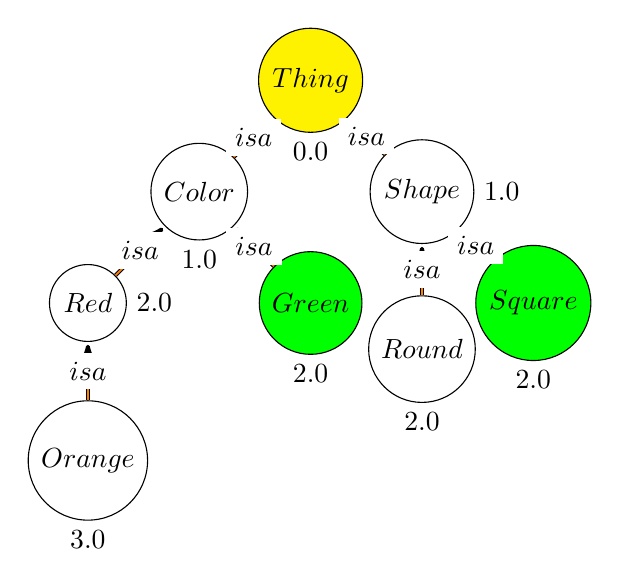
\begin{tikzpicture}[>=stealth',shorten >=1pt,node distance=2cm,on grid,initial/.style    ={}]
          \node[state,fill=yellow,label=below:$0.0$]          (A)                        {$Thing$};
          \node[state,label=below:$1.0$]          (B) [below left =of A]    {$Color$};
          \node[state,label=right:$1.0$]          (C) [below right =of A]    {$Shape$};
          \node[state,label=right:$2.0$]          (D) [below left =of B]    {$Red$};
          \node[state,fill=green,label=below:$2.0$]          (H) [below right =of B]    {$Green$};
          \node[state,label=below:$3.0$]          (E) [below  =of D]    {$Orange$};
          \node[state,label=below:$2.0$]          (F) [below =of C]    {$Round$};
          \node[state,fill=green,label=below:$2.0$]          (G) [below right =of C]    {$Square$};
          \tikzset{mystyle/.style={->,double=orange}} 
          \tikzset{highlight/.style={->,double=green}} 
          \tikzset{every node/.style={fill=white}}
          \path (B)     edge [mystyle]    node   {$isa$} (A)
          (C)     edge [mystyle]    node   {$isa$} (A) 
          (D)     edge [mystyle]    node   {$isa$} (B)
          (H)     edge [mystyle]    node   {$isa$} (B)
          (E)     edge [mystyle]    node   {$isa$} (D)
          (F)     edge [mystyle]    node   {$isa$} (C)
          (G)     edge [mystyle]    node   {$isa$} (C);
          \tikzset{mystyle/.style={<->,double=orange}}   
          \tikzset{mystyle/.style={<->,relative=true,in=0,out=60,double=orange}}
        \end{tikzpicture}
      }
    \end{column}
    \begin{column}{.4\textwidth}
      \begin{itemize}
      \item Resnik 1995: similarity between $x$ and $y$ is the
        information content of the {\em most informative common
          ancestor}
        \item $sim_{Resnik}(Square, Orange) = 0.0$
      \end{itemize}
    \end{column}
  \end{columns}
\end{frame}

\begin{frame}
  \frametitle{How to measure similarity?}
  \begin{itemize}
  \item (Red, Green) and (Orange, Green) have the same similarity
  \item need to incorporate the specificity of the compared classes
  \end{itemize}
\end{frame}

\begin{frame}
  \frametitle{How to measure similarity?}
  \begin{columns}
    \begin{column}{.6\textwidth}
      {\tiny
        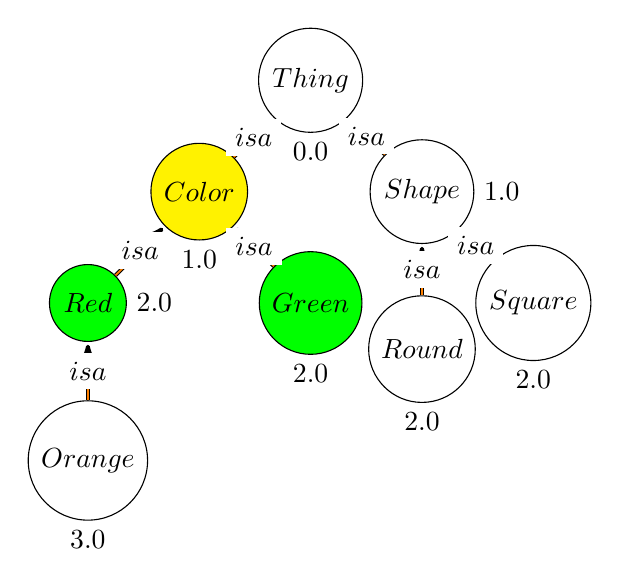
\begin{tikzpicture}[>=stealth',shorten >=1pt,node distance=2cm,on grid,initial/.style    ={}]
          \node[state,label=below:$0.0$]          (A)                        {$Thing$};
          \node[state,fill=yellow,label=below:$1.0$]          (B) [below left =of A]    {$Color$};
          \node[state,label=right:$1.0$]          (C) [below right =of A]    {$Shape$};
          \node[state,fill=green,label=right:$2.0$]          (D) [below left =of B]    {$Red$};
          \node[state,fill=green,label=below:$2.0$]          (H) [below right =of B]    {$Green$};
          \node[state,label=below:$3.0$]          (E) [below  =of D]    {$Orange$};
          \node[state,label=below:$2.0$]          (F) [below =of C]    {$Round$};
          \node[state,label=below:$2.0$]          (G) [below right =of C]    {$Square$};
          \tikzset{mystyle/.style={->,double=orange}} 
          \tikzset{highlight/.style={->,double=green}} 
          \tikzset{every node/.style={fill=white}}
          \path (B)     edge [mystyle]    node   {$isa$} (A)
          (C)     edge [mystyle]    node   {$isa$} (A) 
          (D)     edge [mystyle]    node   {$isa$} (B)
          (H)     edge [mystyle]    node   {$isa$} (B)
          (E)     edge [mystyle]    node   {$isa$} (D)
          (F)     edge [mystyle]    node   {$isa$} (C)
          (G)     edge [mystyle]    node   {$isa$} (C);
          \tikzset{mystyle/.style={<->,double=orange}}   
          \tikzset{mystyle/.style={<->,relative=true,in=0,out=60,double=orange}}
        \end{tikzpicture}
      }
    \end{column}
    \begin{column}{.4\textwidth}
      \begin{itemize}
      \item Lin 1998: $sim_{Lin}(x,y) = \frac{2\cdot
          IC(MICA(x,y))}{IC(x) + IC(y)}$
        \pause
      \item $sim_{Lin}(Green, Red) = 0.5$
      \end{itemize}
    \end{column}
  \end{columns}
\end{frame}

\begin{frame}
  \frametitle{How to measure similarity?}
  \begin{columns}
    \begin{column}{.6\textwidth}
      {\tiny
        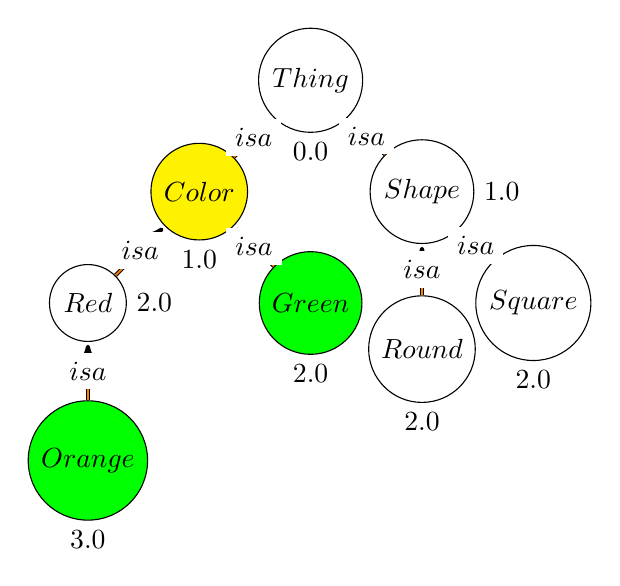
\begin{tikzpicture}[>=stealth',shorten >=1pt,node distance=2cm,on grid,initial/.style    ={}]
          \node[state,label=below:$0.0$]          (A)                        {$Thing$};
          \node[state,fill=yellow,label=below:$1.0$]          (B) [below left =of A]    {$Color$};
          \node[state,label=right:$1.0$]          (C) [below right =of A]    {$Shape$};
          \node[state,label=right:$2.0$]          (D) [below left =of B]    {$Red$};
          \node[state,fill=green,label=below:$2.0$]          (H) [below right =of B]    {$Green$};
          \node[state,fill=green,label=below:$3.0$]          (E) [below  =of D]    {$Orange$};
          \node[state,label=below:$2.0$]          (F) [below =of C]    {$Round$};
          \node[state,label=below:$2.0$]          (G) [below right =of C]    {$Square$};
          \tikzset{mystyle/.style={->,double=orange}} 
          \tikzset{highlight/.style={->,double=green}} 
          \tikzset{every node/.style={fill=white}}
          \path (B)     edge [mystyle]    node   {$isa$} (A)
          (C)     edge [mystyle]    node   {$isa$} (A) 
          (D)     edge [mystyle]    node   {$isa$} (B)
          (H)     edge [mystyle]    node   {$isa$} (B)
          (E)     edge [mystyle]    node   {$isa$} (D)
          (F)     edge [mystyle]    node   {$isa$} (C)
          (G)     edge [mystyle]    node   {$isa$} (C);
          \tikzset{mystyle/.style={<->,double=orange}}   
          \tikzset{mystyle/.style={<->,relative=true,in=0,out=60,double=orange}}
        \end{tikzpicture}
      }
    \end{column}
    \begin{column}{.4\textwidth}
      \begin{itemize}
      \item Lin 1998: $sim_{Lin}(x,y) = \frac{2\cdot
          IC(MICA(x,y))}{IC(x) + IC(y)}$
      \item $sim_{Lin}(Green, Orange) = 0.4$
      \end{itemize}
    \end{column}
  \end{columns}
\end{frame}

\begin{frame}
  \frametitle{How to measure similarity?}
  \begin{itemize}
  \item many(!) others:
    \begin{itemize}
    \item Jiang \& Conrath 1997
    \item Mazandu \& Mulder 2013
    \item Schlicker et al. 2009
    \item ...
  \end{itemize}
  \end{itemize}
\end{frame}

\begin{frame}
  \frametitle{How to measure similarity?}
  \begin{itemize}
  \item we only looked at comparing pairs of classes
  \item mostly, we want to compare {\em sets} of classes
    \begin{itemize}
    \item set of GO annotations
    \item set of signs and symptoms
    \item set of phenotypes
    \end{itemize}
  \item two approaches:
    \begin{itemize}
    \item compare each class individually, then merge
    \item directly set-based similarity measures
    \end{itemize}
  \end{itemize}
\end{frame}

\begin{frame}
  \frametitle{How to measure similarity?}
  \begin{columns}
    \begin{column}{.6\textwidth}
      {\tiny
        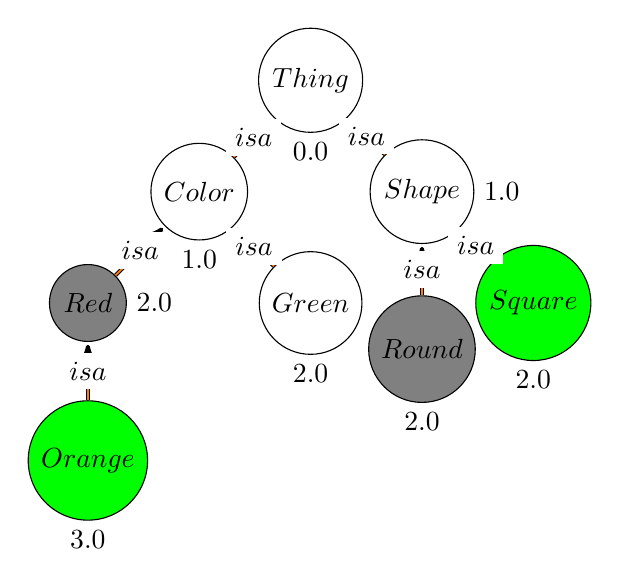
\begin{tikzpicture}[>=stealth',shorten >=1pt,node distance=2cm,on grid,initial/.style    ={}]
          \node[state,label=below:$0.0$]          (A)                        {$Thing$};
          \node[state,label=below:$1.0$]          (B) [below left =of A]    {$Color$};
          \node[state,label=right:$1.0$]          (C) [below right =of A]    {$Shape$};
          \node[state,fill=gray,label=right:$2.0$]          (D) [below left =of B]    {$Red$};
          \node[state,label=below:$2.0$]          (H) [below right =of B]    {$Green$};
          \node[state,fill=green,label=below:$3.0$]          (E) [below  =of D]    {$Orange$};
          \node[state,fill=gray,label=below:$2.0$]          (F) [below =of C]    {$Round$};
          \node[state,fill=green,label=below:$2.0$]          (G) [below right =of C]    {$Square$};
          \tikzset{mystyle/.style={->,double=orange}} 
          \tikzset{highlight/.style={->,double=green}} 
          \tikzset{every node/.style={fill=white}}
          \path (B)     edge [mystyle]    node   {$isa$} (A)
          (C)     edge [mystyle]    node   {$isa$} (A) 
          (D)     edge [mystyle]    node   {$isa$} (B)
          (H)     edge [mystyle]    node   {$isa$} (B)
          (E)     edge [mystyle]    node   {$isa$} (D)
          (F)     edge [mystyle]    node   {$isa$} (C)
          (G)     edge [mystyle]    node   {$isa$} (C);
          \tikzset{mystyle/.style={<->,double=orange}}   
          \tikzset{mystyle/.style={<->,relative=true,in=0,out=60,double=orange}}
        \end{tikzpicture}
      }
    \end{column}
    \begin{column}{.4\textwidth}
      \begin{itemize}
      \item similarity between a square-and-orange thing and a
        round-and-red thing
        \pause
      \item Pesquita et al., 2007:
        $simGIC(X,Y) = \frac{\sum_{c \in A(X) \cap A(Y)}
          IC(c)}{\sum_{c \in A(X) \cup A(Y)} IC(c)}$
      \end{itemize}
    \end{column}
  \end{columns}
\end{frame}

\begin{frame}
  \frametitle{How to measure similarity?}
  \begin{columns}
    \begin{column}{.6\textwidth}
      {\tiny
        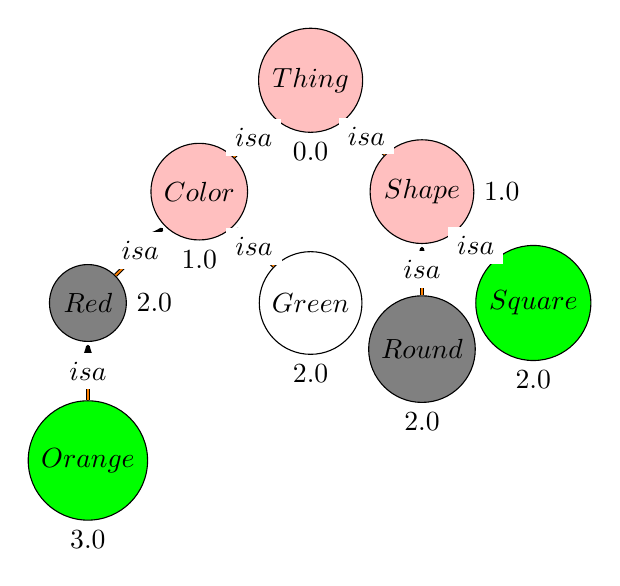
\begin{tikzpicture}[>=stealth',shorten >=1pt,node distance=2cm,on grid,initial/.style    ={}]
          \node[state,fill=pink,label=below:$0.0$]          (A)                        {$Thing$};
          \node[state,fill=pink,label=below:$1.0$]          (B) [below left =of A]    {$Color$};
          \node[state,fill=pink,label=right:$1.0$]          (C) [below right =of A]    {$Shape$};
          \node[state,fill=gray,label=right:$2.0$]          (D) [below left =of B]    {$Red$};
          \node[state,label=below:$2.0$]          (H) [below right =of B]    {$Green$};
          \node[state,fill=green,label=below:$3.0$]          (E) [below  =of D]    {$Orange$};
          \node[state,fill=gray,label=below:$2.0$]          (F) [below =of C]    {$Round$};
          \node[state,fill=green,label=below:$2.0$]          (G) [below right =of C]    {$Square$};
          \tikzset{mystyle/.style={->,double=orange}} 
          \tikzset{highlight/.style={->,double=green}} 
          \tikzset{every node/.style={fill=white}}
          \path (B)     edge [mystyle]    node   {$isa$} (A)
          (C)     edge [mystyle]    node   {$isa$} (A) 
          (D)     edge [mystyle]    node   {$isa$} (B)
          (H)     edge [mystyle]    node   {$isa$} (B)
          (E)     edge [mystyle]    node   {$isa$} (D)
          (F)     edge [mystyle]    node   {$isa$} (C)
          (G)     edge [mystyle]    node   {$isa$} (C);
          \tikzset{mystyle/.style={<->,double=orange}}   
          \tikzset{mystyle/.style={<->,relative=true,in=0,out=60,double=orange}}
        \end{tikzpicture}
      }
    \end{column}
    \begin{column}{.4\textwidth}
      \begin{itemize}
      \item similarity between a square-and-orange thing and a
        round-and-red thing
      \item Pesquita et al., 2007:
        $simGIC(X,Y) = \frac{\sum_{c \in A(X) \cap A(Y)}
          IC(c)}{\sum_{c \in A(X) \cup A(Y)} IC(c)}$
      \item $simGIC(so,rr) = \frac{2}{11}$
      \end{itemize}
    \end{column}
  \end{columns}
\end{frame}

\begin{frame}
  \frametitle{How to measure similarity?}
  \begin{itemize}
  \item alternatively: use different merging strategies
  \item common: average, maximum, {\bf best-matching average}
    \begin{itemize}
    \item Average: $sim_A(X,Y) = \frac{\sum_{x\in X} \sum_{y \in Y} sim(x,y)}{|X| \times |Y|}$
    \item Max average: $sim_{MA}(X,Y) = \frac{1}{|X|} \sum_{x\in X} \max_{y \in Y} sim(x,y)$
    \item Best match average: $sim_{BMA}(X,Y) = \frac{sim_{MA}(X,Y) + sim_{MA}(Y,X)}{2}$
    \end{itemize}
  \end{itemize}
\end{frame}

\begin{frame}
  \frametitle{How to measure similarity?}
  \begin{itemize}
  \item Semantic Measures Library:
    \begin{itemize}
    \item comprehensive Java library
    \item \url{http://www.semantic-measures-library.org/}
    \end{itemize}
  \item R packages: GOSim, GOSemSim, HPOSim, LSAfun,
    ontologySimilarity,...
  \item Python: sematch, fastsemsim (GO only)
  \end{itemize}
\end{frame}

\begin{frame}
  \frametitle{Applications of semantic similarity}
  \begin{block}{Hypothesis}
    Proteins with similar functions are more likely to interact.
  \end{block}
  \begin{itemize}
  \item relies on background knowledge about functions (encoded in GO)
  \item ``similarity'' can mean:
    \begin{itemize}
    \item part of the same pathway
    \item siblings of a common super-class
    \item located in the same location
    \end{itemize}
  \item set-based comparison of GO functions
    \begin{itemize}
    \item single GO hierarchy or all?
    \item which similarity measure?
    \end{itemize}
  \end{itemize}
\end{frame}

\begin{frame}
  \frametitle{Applications of semantic similarity}
  \centerline{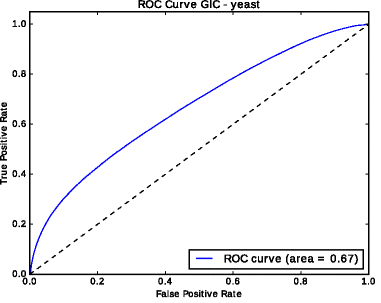
\includegraphics[width=.8\textwidth]{ppi1.png}}
\end{frame}

\begin{frame}
  \frametitle{Applications of semantic similarity}
  \centerline{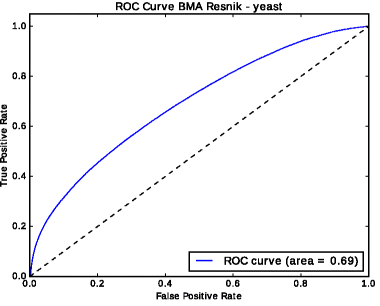
\includegraphics[width=.8\textwidth]{ppi2.png}}
\end{frame}

\begin{frame}
  \frametitle{Applications of semantic similarity}
  \centerline{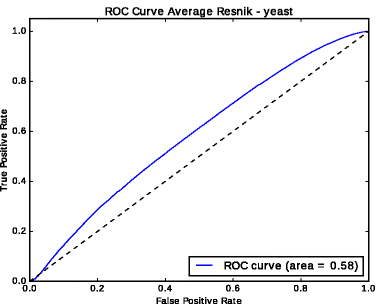
\includegraphics[width=.8\textwidth]{ppi3.png}}
\end{frame}

\begin{frame}
  \frametitle{Applications of semantic similarity}
  \begin{itemize}
  \item no obvious choice of similarity measure
  \item depends on application
    \begin{itemize}
    \item predicting PPIs in different organisms may benefit from a
      different similarity measure!
    \end{itemize}
  \item different similarity measures may react differently to biases
    in data
  \item needs some testing and experience
  \end{itemize}
\end{frame}

\begin{frame}
  \frametitle{Applications of semantic similarity}
  Recommendations for using semantic similarity::
  \begin{itemize}
  \item use Resnik's information content measure
  \item use Resnik's similarity
  \item use Best Match Average
  \item use the full ontology
  \item classify your ontology using a reasoner before applying
    semantic similarity
    \begin{itemize}
    \item although many ontologies come pre-classified
    \end{itemize}
  \item $\Rightarrow$ but there are many exceptions
    \begin{itemize}
    \item similar location $\Rightarrow$ use location subset of GO
    \item developmental phenotypes $\Rightarrow$ use developmental
      branch of phenotype ontology
    \end{itemize}
  \end{itemize}
\end{frame}

\begin{frame}
  \frametitle{Applications of semantic similarity}
  \begin{itemize}
  \item choice of ontology determines the kind of similarity
  \item functional similarity: Gene Ontology
  \item anatomical, structural similarity: anatomy ontologies (Uberon,
    MA, FMA, etc.)
  \item phenotypic similarity: phenotype ontology (HPO, MP, etc.)
  \item chemical structural similarity: ChEBI
  \end{itemize}
\end{frame}

\begin{frame}
  \frametitle{Applications of semantic similarity}
  \begin{itemize}
  \item phenotypic similarity used to:
    \begin{itemize}
    \item diagnosis: similarity between patient phenotypes and disease
      phenotypes
      \begin{itemize}
      \item also between patient phenotypes, e.g., Phenomizer:
        \url{http://compbio.charite.de/phenomizer/}
      \end{itemize}
    \item disease modules: similarity between disease and disease
    \item clustering/stratification: similarity between patient and patient
    \item disease gene discovery: similarity between patient/disease
      phenotypes and gene--phenotype associations
      \begin{itemize}
      \item in humans
      \item in model organisms
      \end{itemize}
    \item drug repurposing: side-effect similarity; similarity between
      side effect profile and gene--disease associations
    \end{itemize}
  \end{itemize}
\end{frame}

\begin{frame}
  \frametitle{Applications of semantic similarity}
  \begin{itemize}
  \item comparing entities annotated with {\em different}
    ontologies/vocabularies of the {\em same} (or related) domains
    \begin{itemize}
    \item medical: UMLS, HPO, DO, ORDO, NCIT, ICD, SNOMED CT, MeSH, ...
    \item phenotype: HPO, MP, CPO, WBPhenotype, FBCV, MeSH, ...
    \item chemical: ChEBI, MeSH, DrOn, RXNorm, DrugBank, ...
    \end{itemize}
  \end{itemize}
\end{frame}

\begin{frame}
  \frametitle{Applications of semantic similarity}
  \begin{itemize}
  \item needs mapping, alignment, or integration
    \begin{itemize}
    \item mapping: given a term $t$, find corresponding class in
      ontology $O$
      \begin{itemize}
      \item can be 1:1, 1:n, n:1, n:m
      \item $t$ can be from ontology, vocabulary, database, or text
      \item use $O$ for analysis
      \end{itemize}
    \item alignment: given two ontologies or vocabularies $O_1$ and
      $O_2$, find all mappings between classes/terms in $O_1$ and $O_2$
      \begin{itemize}
      \item applicable to ontologies and vocabularies
      \item use $O_1$ or $O_2$ for analysis
      \end{itemize}
    \item integration: given two ontologies $O_1$ and $O_2$, combine
      both ontologies into a single ontology $O$
      \begin{itemize}
      \item maintain meaning of classes
      \item use $O$ for analysis
      \end{itemize}
    \end{itemize}
  \end{itemize}
\end{frame}

\begin{frame}
  \frametitle{Applications of semantic similarity}
  \begin{itemize}
  \item lexical mappings: use class labels (and synonyms) to find matches
    \begin{itemize}
    \item hypertension ({\tt HP:0000822}) and hypertension ({\tt MP:0000231})
    \end{itemize}
  \item semantic mappings: use class axioms to find matches
    \begin{itemize}
    \item pulmonary valve stenosis ({\tt MP:0006182}) and Pulmonic
      stenosis ({\tt HP:0001642})
    \item both definitions based on constricted ({\tt PATO:0001847})
      and pulmonary valve ({\tt UBERON:0002146})
    \end{itemize}
  \item hybrid: combine lexical and semantic mappings
  \end{itemize}
\end{frame}

\begin{frame}
  \frametitle{Applications of semantic similarity}
  tools for ontology mapping, matching, integration:
  \begin{itemize}
  \item AgreementMaker Light: \url{https://github.com/AgreementMakerLight/AML-Jar}
    \begin{itemize}
    \item structural (semantic) and lexical matches
    \item can use domain-specific background knowledge
    \end{itemize}
  \item LogMap: \url{https://github.com/ernestojimenezruiz/logmap-matcher}
    \begin{itemize}
    \item structural (semantic) and lexical matches
    \item biology-themed versions
    \end{itemize}
  \item NCBO Annotator: \url{https://bioportal.bioontology.org/annotator}
    \begin{itemize}
    \item lexical matches only
    \item can annotate full text
    \end{itemize}
  \item recent tools and comprehensive ongoing evaluation:
    \begin{itemize}
    \item OAEI: \url{http://oaei.ontologymatching.org/}
    \end{itemize}
  \end{itemize}
\end{frame}

\begin{frame}
  \frametitle{Hands-on part: diagnosing rare disease using mouse phenotypes}
  \begin{itemize}
  \item run the ``Semantic Similarity'' notebook
    \begin{itemize}
    \item then find the mouse genotype with the most similar set of
      phenotypes to ``Tetralogy of Fallot'' ({\tt OMIM:187500})
    \item or: use the data from
      \url{https://hpo.jax.org/app/download/annotation} to add more
      diseases and query by disease (hint: a disease is really just a
      set of phenotypes)
    \end{itemize}
  \end{itemize}
\end{frame}

\end{document}
%%% Local Variables:
%%% mode: latex
%%% TeX-master: t
%%% End:
